\documentclass[aspectratio=169,11pt]{beamer}
\usepackage[fontset=none]{ctex}
\usepackage{amsmath}
\usepackage{booktabs}
\usepackage{tikz}
\usetikzlibrary{arrows.meta,calc}
\usefonttheme[onlymath]{serif}
\setCJKsansfont{Microsoft YaHei}
\setCJKmainfont{Microsoft YaHei}
\setsansfont{Segoe UI}
\setmonofont{Consolas}
\graphicspath{{figures/}}

\definecolor{paper}{HTML}{F7F4EC}
\definecolor{ink}{HTML}{1C1B19}
\definecolor{muted}{HTML}{6B6860}
\definecolor{faint}{HTML}{C9C5B9}
\definecolor{sand}{HTML}{D9D5C8}
\definecolor{zblue}{HTML}{2A78D6}
\definecolor{zorange}{HTML}{EB6834}
\definecolor{grayE}{HTML}{8F8A7C}
\definecolor{grayT}{HTML}{514E47}

\setbeamercolor{background canvas}{bg=paper}
\setbeamercolor{normal text}{fg=ink}
\setbeamercolor{frametitle}{fg=ink}
\setbeamercolor{structure}{fg=ink}
\setbeamertemplate{navigation symbols}{}
\setbeamersize{text margin left=12mm,text margin right=12mm}
\setbeamertemplate{frametitle}{\vspace*{7mm}\parbox{\textwidth}{\fontsize{17.5}{23}\selectfont\bfseries\insertframetitle}\vspace*{1mm}}

% 页脚是一条 Z 峰形状的曲线，圆点随页码移动，峰顶正好落在"悬崖"那一页
\newcommand{\mainframes}{12}
\setbeamertemplate{footline}{%
  \begin{tikzpicture}[x=1mm,y=1mm]
    \useasboundingbox (0,0) rectangle (160,8);
    \draw[faint,line width=.5pt] plot[domain=0:1,samples=160,smooth] ({12+\x*128},{1.6+4.4/(1+((\x-.636)/.022)^2)});
    \pgfmathsetmacro{\prog}{min(1,(\insertframenumber-1)/(\mainframes-1))}
    \fill[zorange] ({12+\prog*128},{1.6+4.4/(1+((\prog-.636)/.022)^2)}) circle (.75);
    \node[anchor=east,text=muted,font=\fontsize{7}{8}\selectfont] at (150,2) {\insertframenumber};
  \end{tikzpicture}}

\newcommand{\smallnote}[1]{{\fontsize{9}{12.5}\selectfont\color{muted}#1}}
\newcommand{\bignum}[1]{{\fontsize{27}{31}\selectfont\bfseries #1}}
\newcommand{\hl}[1]{{\color{zorange}\bfseries #1}}
\newcommand{\pT}{p_{\mathrm{T}}}
\newcommand{\mll}{m_{\mu\mu}}
\newcommand{\swatch}[1]{\tikz[baseline=0.2ex]\fill[#1] (0,0) rectangle (2.6mm,2.6mm);}
\newcommand{\qitem}[2]{\begin{tikzpicture}[baseline=(n.base)]\node[inner sep=0,font=\fontsize{24}{24}\selectfont\bfseries,text=zorange] (n) {#1};\end{tikzpicture}\hspace{5mm}\parbox[t]{118mm}{\fontsize{13.5}{19}\selectfont #2}\par\vspace{7.5mm}}

\begin{document}
\setlength{\parindent}{0pt}

% 1 ---------------------------------------------------------------------
{\setbeamertemplate{footline}{}
\begin{frame}[plain]
  \vspace*{4mm}
  {\fontsize{30}{39}\selectfont\bfseries 如何用一行代码\\杀死一个 Z 玻色子\par}
  \vspace{2mm}
  {\fontsize{12}{16}\selectfont\color{muted}在 ATLAS Open Data 里做一次 $\pT$ 阈值实验\par}
  \vspace{1.5mm}
  {\fontsize{10}{14}\selectfont\color{muted}唐同舟\quad 复旦大学物理学系\quad 暗物质课题学习组\par}
  \vspace{3mm}
  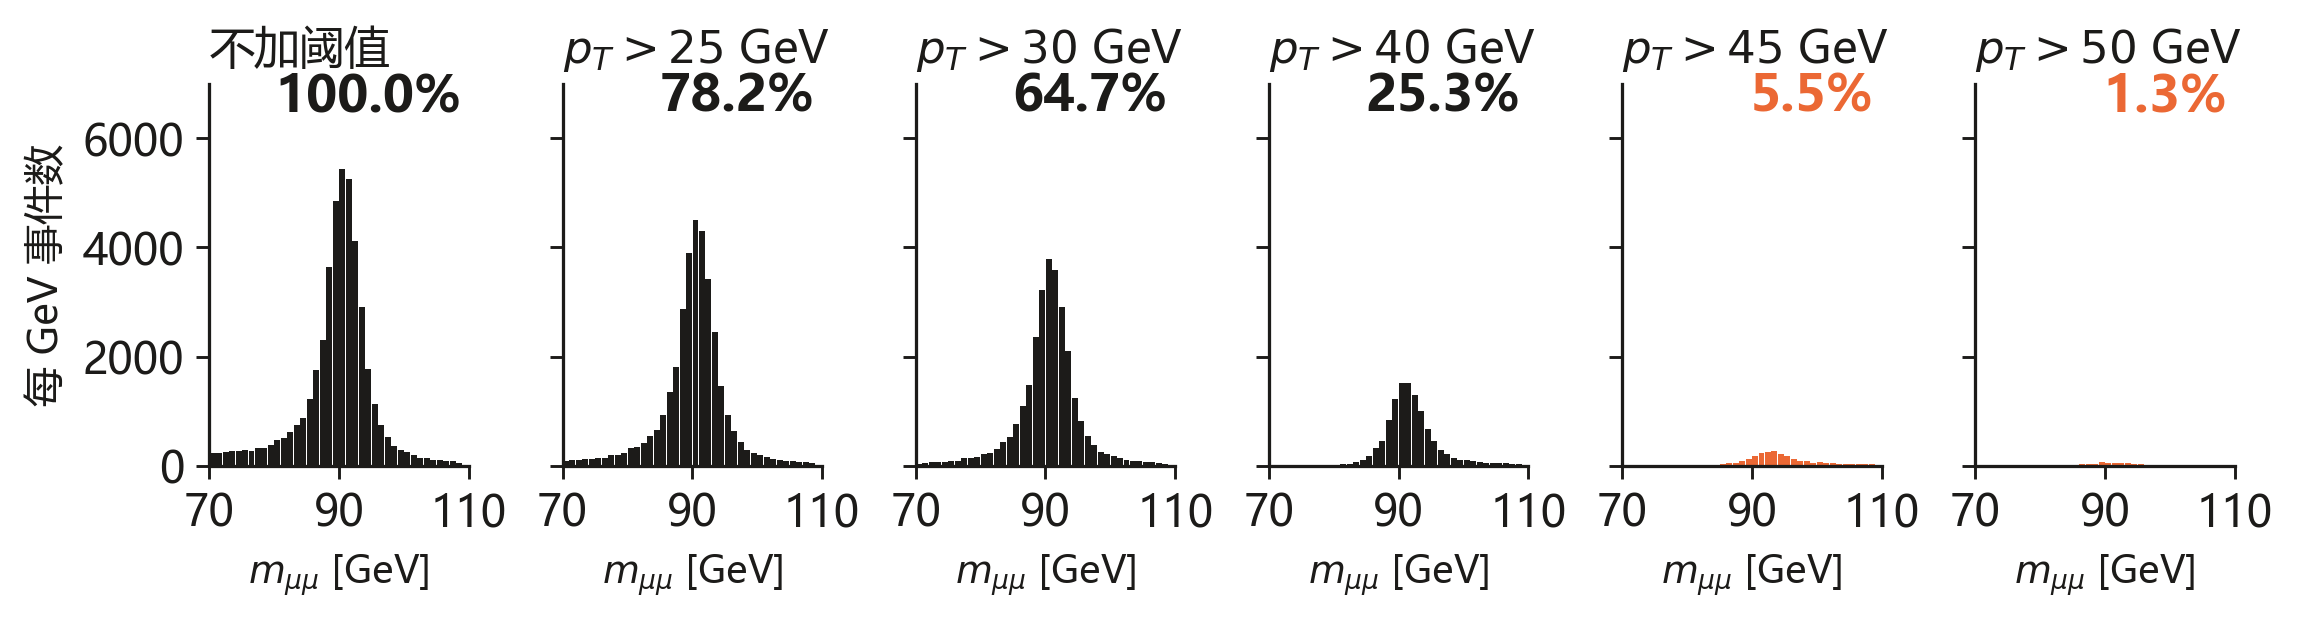
\includegraphics[width=\textwidth]{filmstrip.png}
\end{frame}
}

% 2 ---------------------------------------------------------------------
\begin{frame}{Z 已经死了。探测器里只剩下两个 μ 子}
  \begin{columns}[T,totalwidth=\textwidth]
    \begin{column}{.47\textwidth}
      \vspace{-3mm}\centering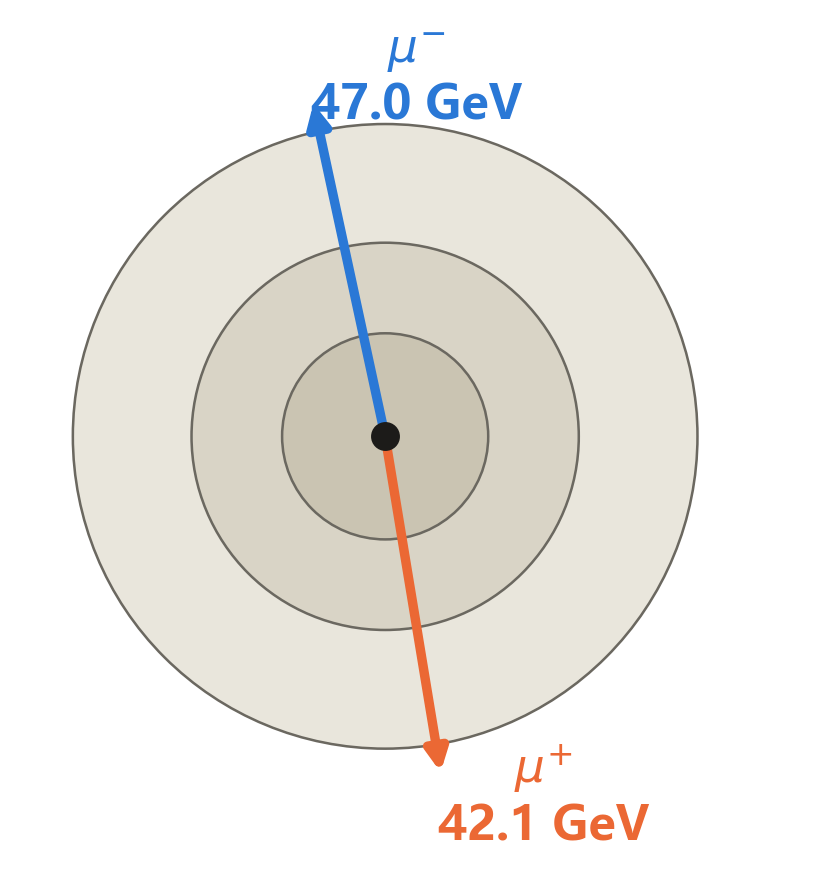
\includegraphics[height=56mm]{event_display.png}
    \end{column}
    \begin{column}{.51\textwidth}
      \vspace{-1mm}
      {\small\bfseries 一次真实对撞\quad\mdseries\color{muted} 事件号 1569374}\par\vspace{2.5mm}
      {\small\begin{tabular}{@{}lrrrr@{}}
        \toprule
        & $\pT$ [GeV] & $\eta$ & $\phi$ & $E$ [GeV]\\
        \midrule
        {\color{zblue}$\mu^-$} & 46.98 & 0.52 & 1.78 & 53.59\\
        {\color{zorange}$\mu^+$} & 42.13 & 0.07 & $-1.41$ & 42.23\\
        \bottomrule
      \end{tabular}\par}
      \vspace{4mm}
      {\small Z 的寿命只有约 $2.6\times10^{-25}$ s。\par\vspace{1mm}
      $c\tau\approx0.08$ fm，比质子半径还短，\\还没离开对撞点就衰变了。\par}
      \vspace{4mm}
      {\small\bfseries 我们手里只有这四个数乘二。\par}
      \vspace{4mm}
      \smallnote{箭头方向来自真实数据。圆环由内到外：径迹室、量能器、μ 子谱仪（示意，不按比例）。}
    \end{column}
  \end{columns}
\end{frame}

% 3 ---------------------------------------------------------------------
\begin{frame}{只要一个不随参考系改变的量，就能认出它}
  \begin{columns}[T,totalwidth=\textwidth]
    \begin{column}{.56\textwidth}
      \vspace{3mm}
      \[\mll^2=(E_1+E_2)^2-\lvert\vec p_1+\vec p_2\rvert^2\]\par
      \vspace{1mm}
      {\small 代入刚才那个事件：\par\vspace{2mm}
      $E=53.59+42.23=95.82$ GeV\par\vspace{1mm}
      $\lvert\vec p_1+\vec p_2\rvert=29.14$ GeV\par\vspace{3mm}}
      \[\mll=\sqrt{95.82^2-29.14^2}=\textcolor{zorange}{\mathbf{91.28\ \mathrm{GeV}}}\]\par
      \vspace{2mm}
      {\small 每个 μ 子只有 0.106 GeV，合起来却是 91 GeV：\\质量不能简单相加。\par}
    \end{column}
    \begin{column}{.42\textwidth}
      \centering\vspace{3mm}
      % 三角形按真实比例：斜边 E，两条直角边 m 和 |p|
      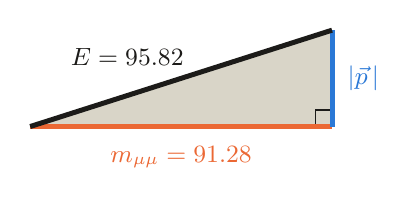
\begin{tikzpicture}[x=0.42mm,y=0.42mm]
        \coordinate (A) at (0,0);
        \coordinate (B) at (91.28,0);
        \coordinate (C) at (91.28,29.14);
        \fill[sand] (A)--(B)--(C)--cycle;
        \draw[ink,line width=.6pt] (B)+(-5,0)--+(-5,5)--+(0,5);
        \draw[zorange,line width=1.8pt] (A)--(B) node[midway,below=1mm,font=\small\bfseries] {$\mll=91.28$};
        \draw[zblue,line width=1.8pt] (B)--(C) node[midway,right=.5mm,font=\small\bfseries] {$\lvert\vec p\,\rvert$};
        \draw[ink,line width=1.8pt] (A)--(C) node[midway,above left=.2mm,font=\small\bfseries,xshift=2mm] {$E=95.82$};
      \end{tikzpicture}\par\vspace{7mm}
      \raggedright
      {\small $m^2=E^2-p^2$ 就是一个直角三角形（图按比例画）。\par\vspace{2mm}
      Z 飞得快慢只改变 $E$ 和 $p$，\\橙色这条边不变。\par}
    \end{column}
  \end{columns}
\end{frame}

% 4 ---------------------------------------------------------------------
\begin{frame}{一个事件只是故事，十几万个事件才是证据}
  \vspace{6mm}
  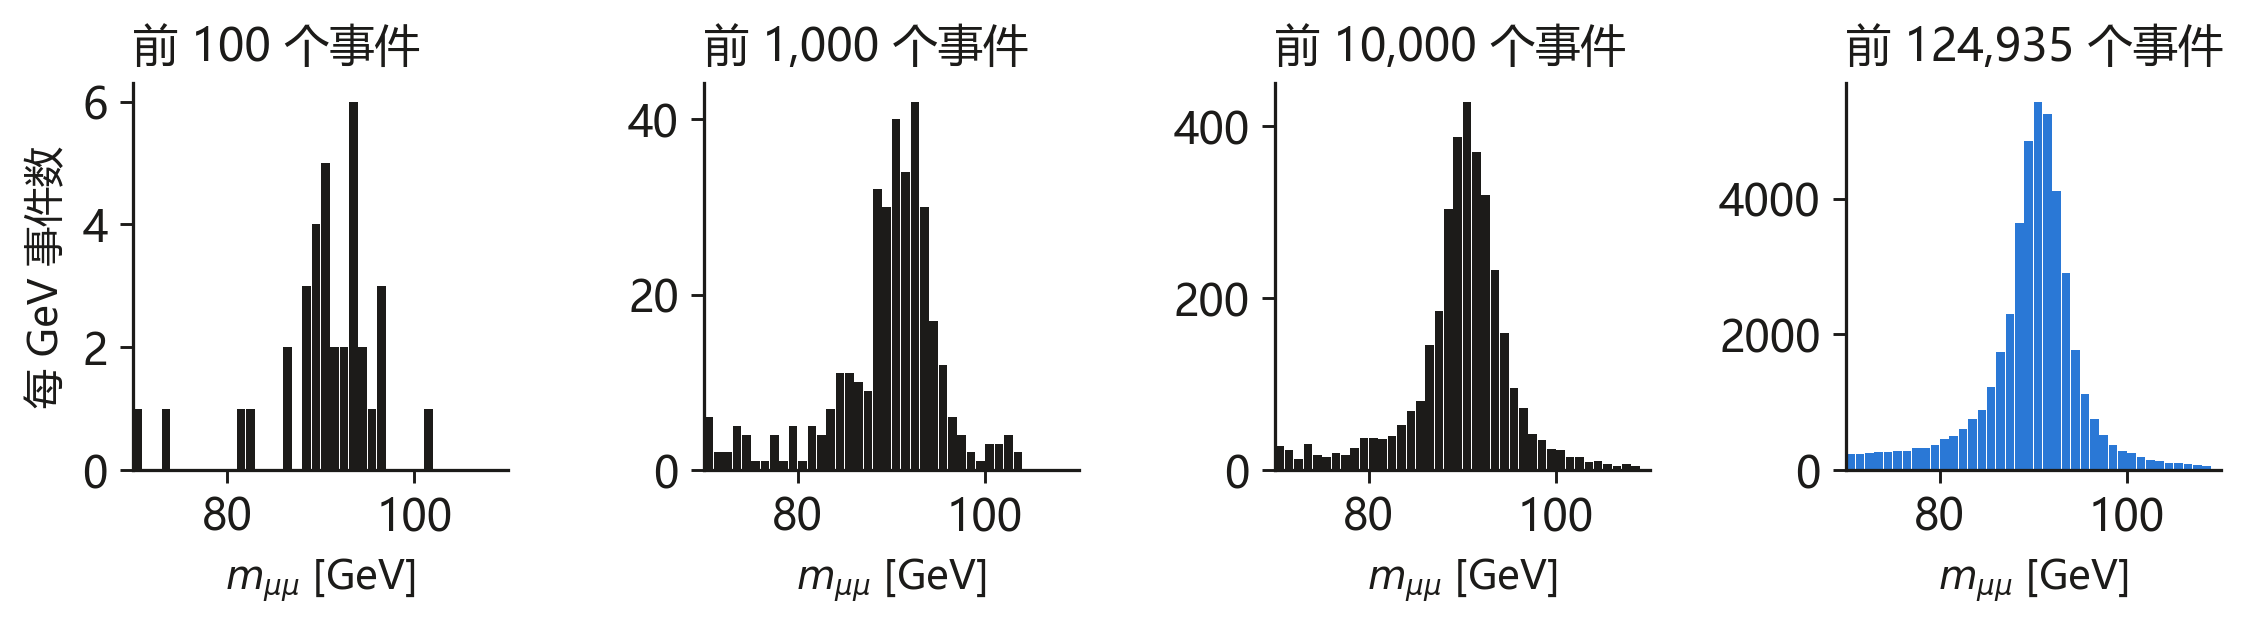
\includegraphics[width=\textwidth]{emergence.png}
  \vspace{7mm}
  \smallnote{同一个数据文件，只是按顺序累积；各图纵轴范围不同。每个事件都只贡献一个数：它的 $\mll$。}
\end{frame}

% 5 ---------------------------------------------------------------------
\begin{frame}{把横轴放开：Z 只是这张谱上的一个峰}
  \vspace{1mm}
  \centering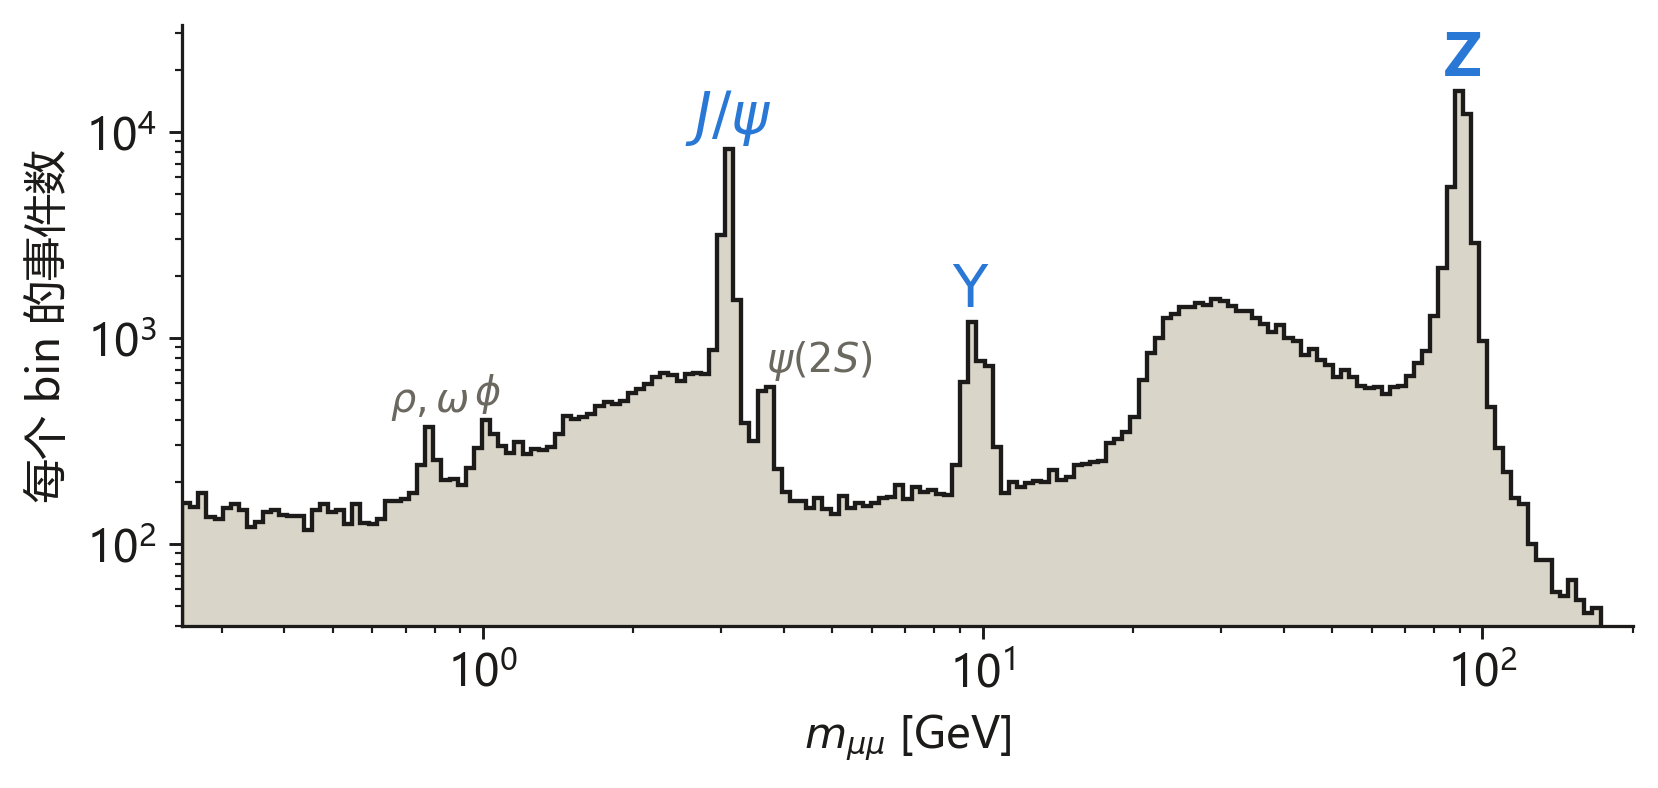
\includegraphics[width=.84\textwidth]{spectrum.png}\par
  \vspace{2mm}\raggedright
  \smallnote{124935 个事件的双 μ 子质量谱。粒子标注是按已知质量给的，这次没有单独验证低质量峰。}
\end{frame}

% 6 ---------------------------------------------------------------------
\begin{frame}{跑通之后才发现：“前两个轻子”不一定是 μ 子}
  \begin{columns}[T,totalwidth=\textwidth]
    \begin{column}{.63\textwidth}
      \vspace{0mm}
      {\small\color{muted} 真实事件的轻子数组，按存储顺序\par}\vspace{1mm}
      \begin{tikzpicture}[x=1mm,y=1mm,box/.style={draw=ink,line width=.6pt,minimum width=21mm,minimum height=11mm,align=center,font=\small}]
        \node[box,fill=sand] (a) at (0,0) {$e$\\7.4 GeV};
        \node[box,fill=white] (b) at (25,0) {$\mu$\\40.4 GeV};
        \node[box,fill=white] (c) at (50,0) {$\mu$\\36.9 GeV};
        \draw[zorange,line width=1.5pt] (-10.5,6.8)--(-10.5,9)--(35.5,9)--(35.5,6.8);
        \node[anchor=south west,text=zorange,font=\small\bfseries,inner xsep=0] at (-10.5,9.4) {notebook 取 lep[0] + lep[1]：14.9 GeV};
        \draw[zblue,line width=1.5pt] (14.5,-6.8)--(14.5,-9)--(60.5,-9)--(60.5,-6.8);
        \node[anchor=north west,text=zblue,font=\small\bfseries,inner xsep=0] at (14.5,-9.4) {实际的 μ 子对：93.5 GeV};
      \end{tikzpicture}\par
      \vspace{4mm}
      {\small 轻子数组里混有电子，也不按 $\pT$ 排序。\\skim 也不是“恰好两个 μ 子”，而是至少两个。\par}
    \end{column}
    \begin{column}{.33\textwidth}
      \vspace{0mm}
      \bignum{\color{zorange}6.3\%}\par\vspace{1mm}
      {\small 7918 / 124935 个事件\\前两个轻子不都是 μ 子\par}
      \vspace{4mm}
      {\small\bfseries 但峰照样在，\\只看图发现不了。\par}
      \vspace{4mm}
      {\small 修正：\texttt{lep\_type == 13}\\窗口内事件 43084 → 43493\par}
    \end{column}
  \end{columns}
\end{frame}

% 7 ---------------------------------------------------------------------
\begin{frame}[fragile]{实验：只加一行代码，把阈值一格一格调高}
  \vspace{3mm}
  \begin{tikzpicture}
    \node[fill=ink,text=paper,inner xsep=4mm,inner ysep=2.5mm,font=\ttfamily\small] {mask = np.all(pt > cut, axis=1)\ \ \ \# 两个 μ 子都要过线};
  \end{tikzpicture}\par
  \vspace{3mm}
  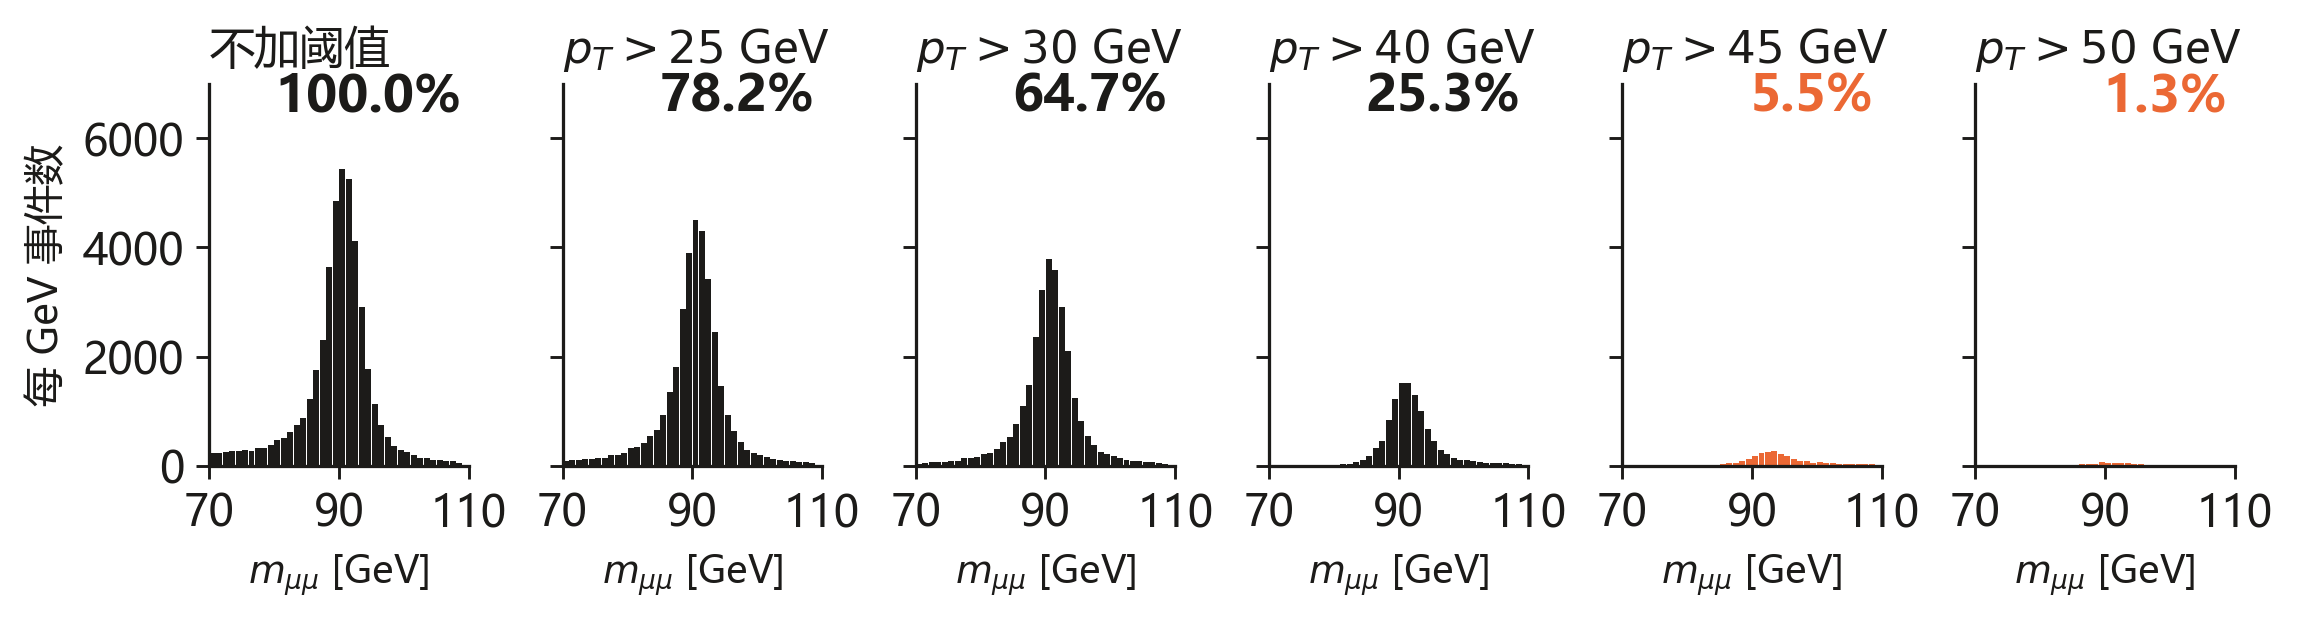
\includegraphics[width=\textwidth]{filmstrip.png}\par
  \vspace{1mm}
  \smallnote{百分比是 70--109 GeV 内留下的事件比例。纵轴相同，高度可以直接比。}
\end{frame}

% 8 ---------------------------------------------------------------------
\begin{frame}{45.6 GeV 是悬崖的边缘，不是巧合}
  \vspace{1mm}
  \centering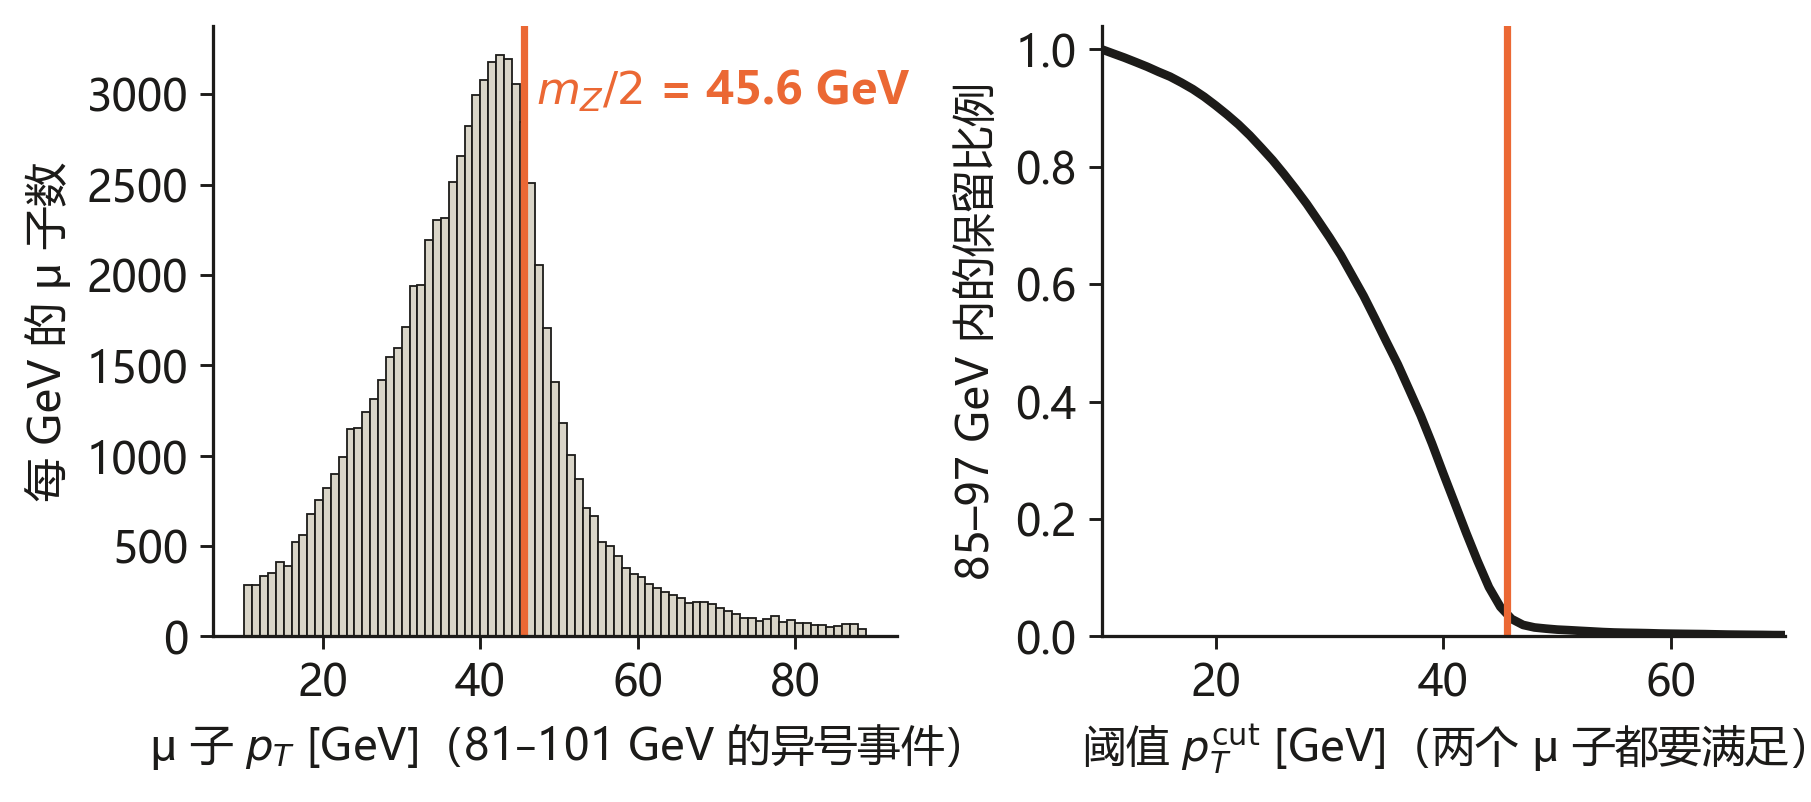
\includegraphics[width=.8\textwidth]{cliff.png}\par
  \vspace{1mm}\raggedright
  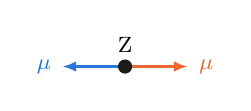
\begin{tikzpicture}[x=1mm,y=1mm,baseline=-1mm]
    \draw[-{Latex[length=1.8mm]},zblue,line width=1.3pt] (0,0)--(-8,0) node[left,font=\footnotesize] {$\mu$};
    \draw[-{Latex[length=1.8mm]},zorange,line width=1.3pt] (0,0)--(8,0) node[right,font=\footnotesize] {$\mu$};
    \fill[ink] (0,0) circle (.9);
    \node[above,font=\footnotesize] at (0,.6) {Z};
  \end{tikzpicture}\quad
  {\small Z 静止时，每个 μ 子的动量都是 $m_Z/2$。要过 45.6 GeV 这条线，\\Z 就得被额外推一把，或者本身质量更高。\par}
\end{frame}

% 9 ---------------------------------------------------------------------
\begin{frame}{峰开始移动，而且它会骗人}
  \vspace{1mm}
  \centering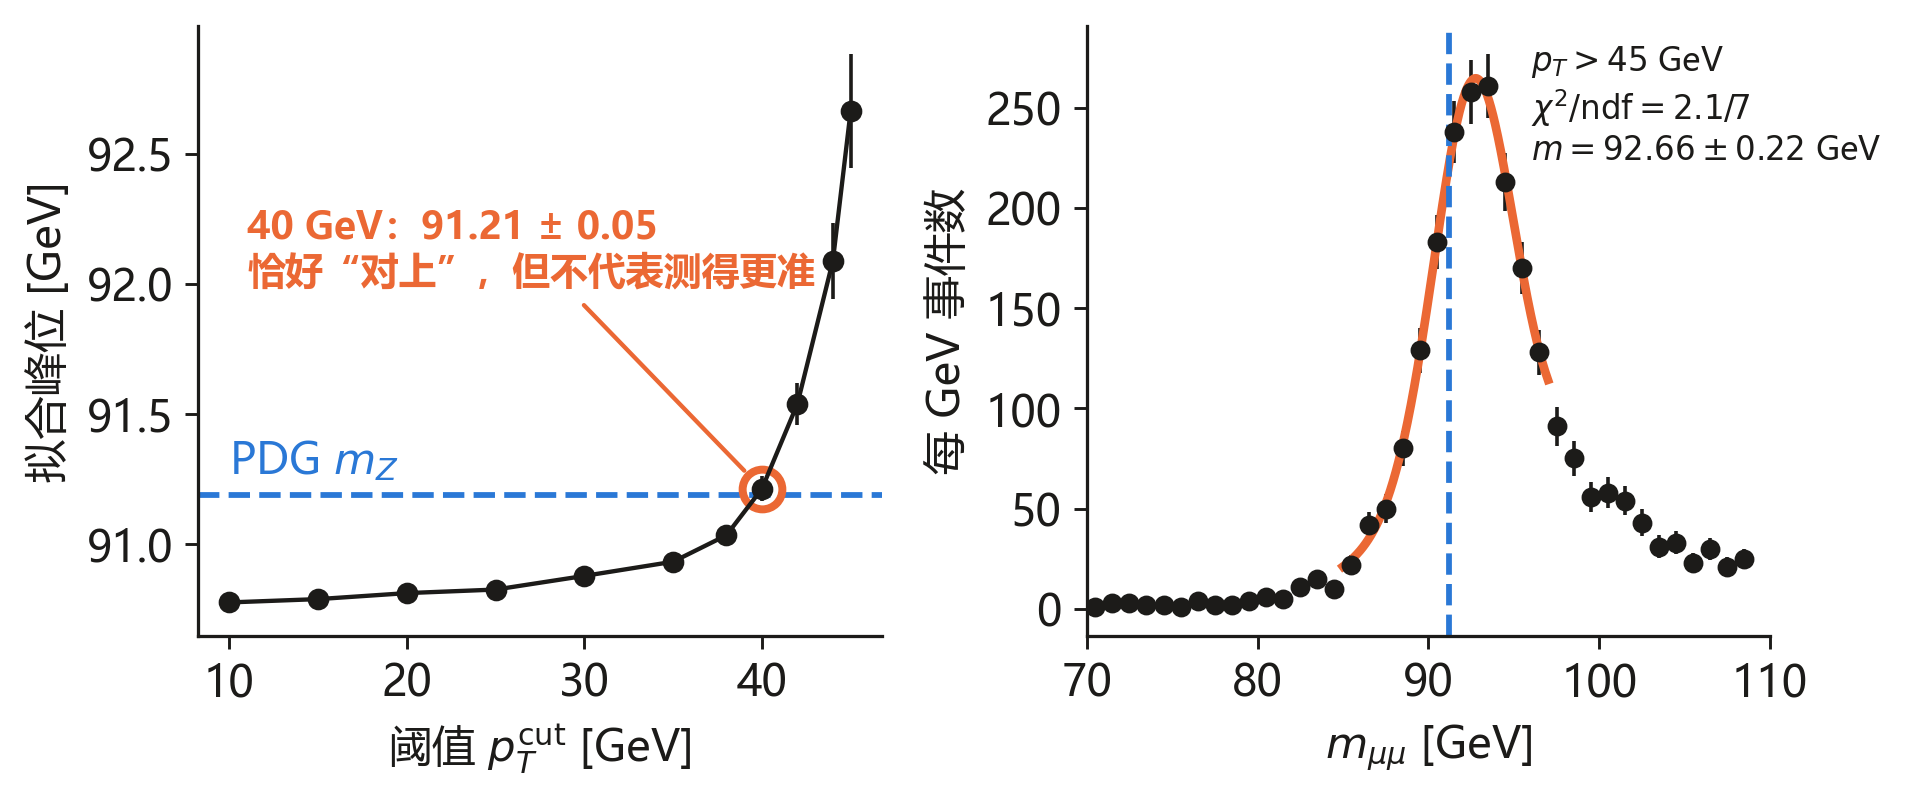
\includegraphics[width=.8\textwidth]{drift_trap.png}\par
  \vspace{1mm}\raggedright
  \begin{columns}[T,totalwidth=\textwidth]
    \begin{column}{.49\textwidth}{\small\bfseries 第一个陷阱\par\mdseries 40 GeV 时几乎等于 PDG 值，但这只是峰在上移途中恰好穿过了它。\par}\end{column}
    \begin{column}{.49\textwidth}{\small\bfseries 第二个陷阱\par\mdseries 45 GeV 时 $\chi^2$ 很漂亮，但事件少、分布已被切变形。$\chi^2$ 好不等于物理对。\par}\end{column}
  \end{columns}
\end{frame}

% 10 --------------------------------------------------------------------
\begin{frame}{两个差异：一个能解释，一个还解释不了}
  \begin{columns}[T,totalwidth=\textwidth]
    \begin{column}{.57\textwidth}
      \vspace{1mm}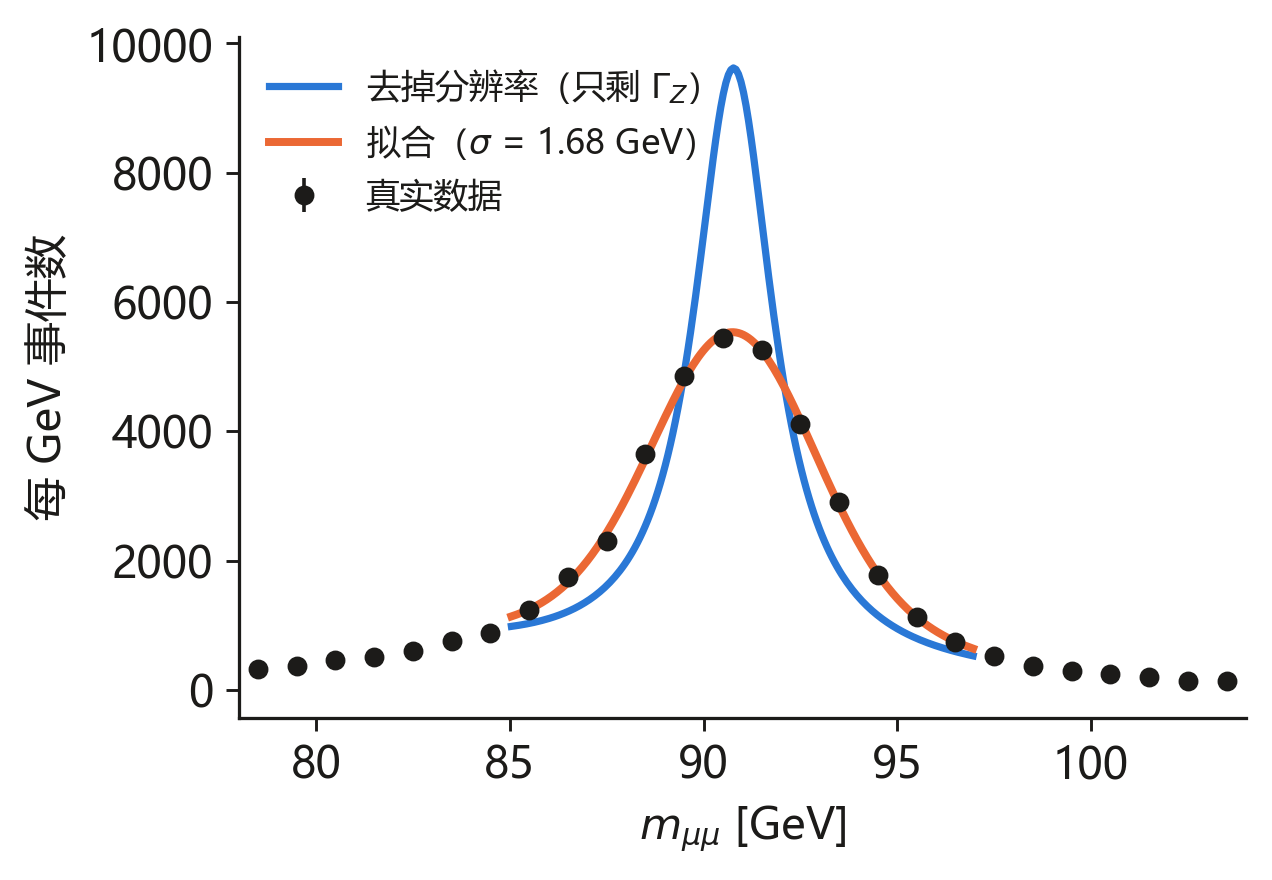
\includegraphics[width=\textwidth]{blur.png}
    \end{column}
    \begin{column}{.40\textwidth}
      \vspace{2mm}
      {\small\bfseries 峰比理论宽\par\vspace{1mm}\mdseries
      全宽约 5.4 GeV，而 $\Gamma_Z=2.50$ GeV。\\探测器分辨率 $\sigma\approx1.7$ GeV 把它抹宽了。\par}
      \vspace{5mm}
      {\small\bfseries 峰比已知值低\par\vspace{1mm}\mdseries
      $90.78\pm0.02$ GeV（仅统计误差），\\PDG 是 91.19 GeV，差 \hl{0.41 GeV}。\par\vspace{1.5mm}
      末态辐射？动量标度？\par\vspace{1.5mm}
      \textbf{只靠数据分不开}，需要模拟和校准。\par}
    \end{column}
  \end{columns}
\end{frame}

% 11 --------------------------------------------------------------------
\begin{frame}{只用了 Z 的 3.4\%；暗物质搜寻盯着“看不见”}
  \begin{columns}[T,totalwidth=\textwidth]
    \begin{column}{.5\textwidth}
      \vspace{-2mm}
      \begin{tikzpicture}
        \node[inner sep=0] (w) {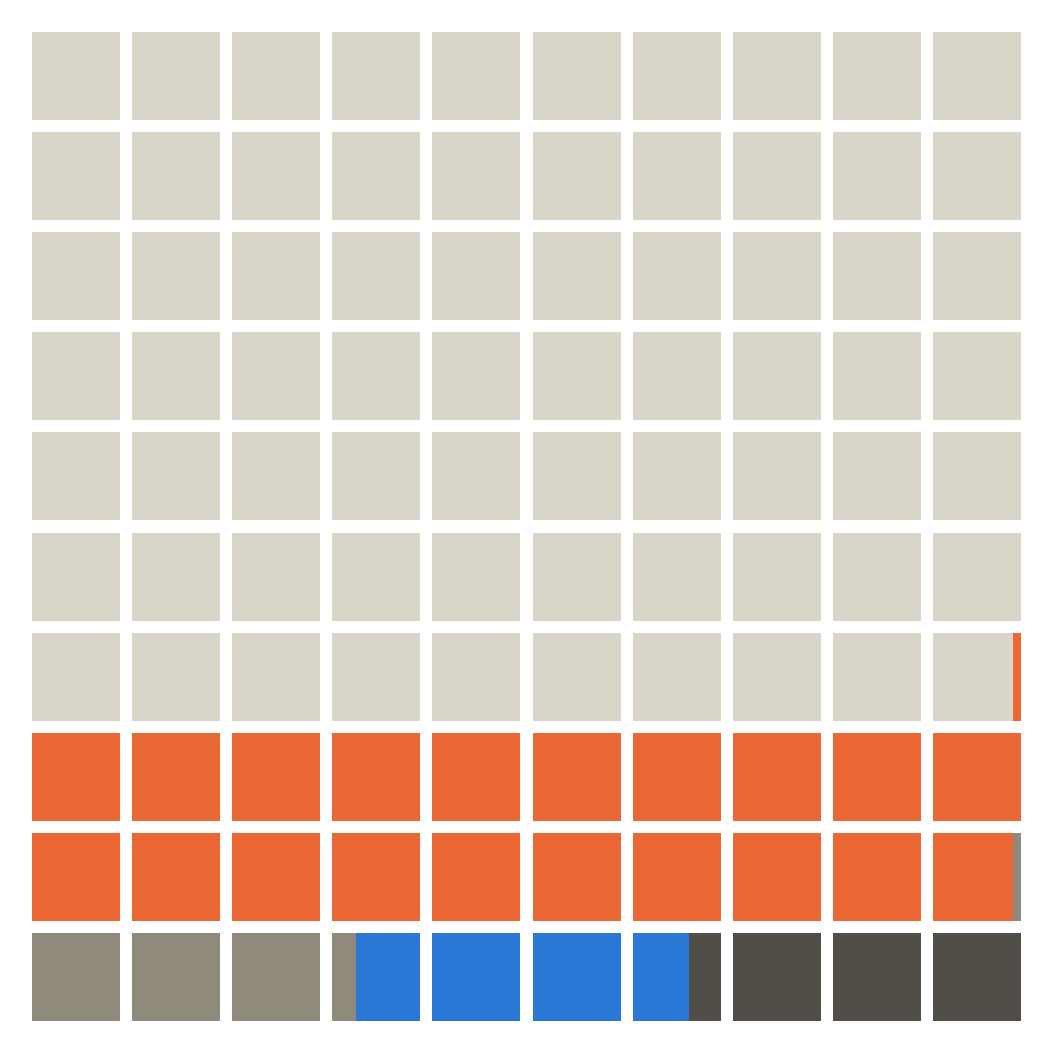
\includegraphics[height=38mm]{waffle.png}};
        \node[anchor=north west,inner sep=0,font=\fontsize{9}{12.5}\selectfont,align=left] at ($(w.north east)+(2.5mm,-1mm)$) {%
          \swatch{sand} 强子 69.9\%\\[.7mm]
          \swatch{zorange} 不可见 20.0\%\\[.7mm]
          \swatch{grayE} $e^+e^-$ 3.4\%\\[.7mm]
          \swatch{zblue} \textbf{$\mu^+\mu^-$ 3.4\%}\\[.7mm]
          \swatch{grayT} $\tau^+\tau^-$ 3.4\%};
      \end{tikzpicture}\par
      \vspace{1.5mm}
      \smallnote{Z 的衰变分支比（PDG 2024），每格 1\%。不可见部分在标准模型中对应中微子对。}
    \end{column}
    \begin{column}{.46\textwidth}
      \vspace{-2mm}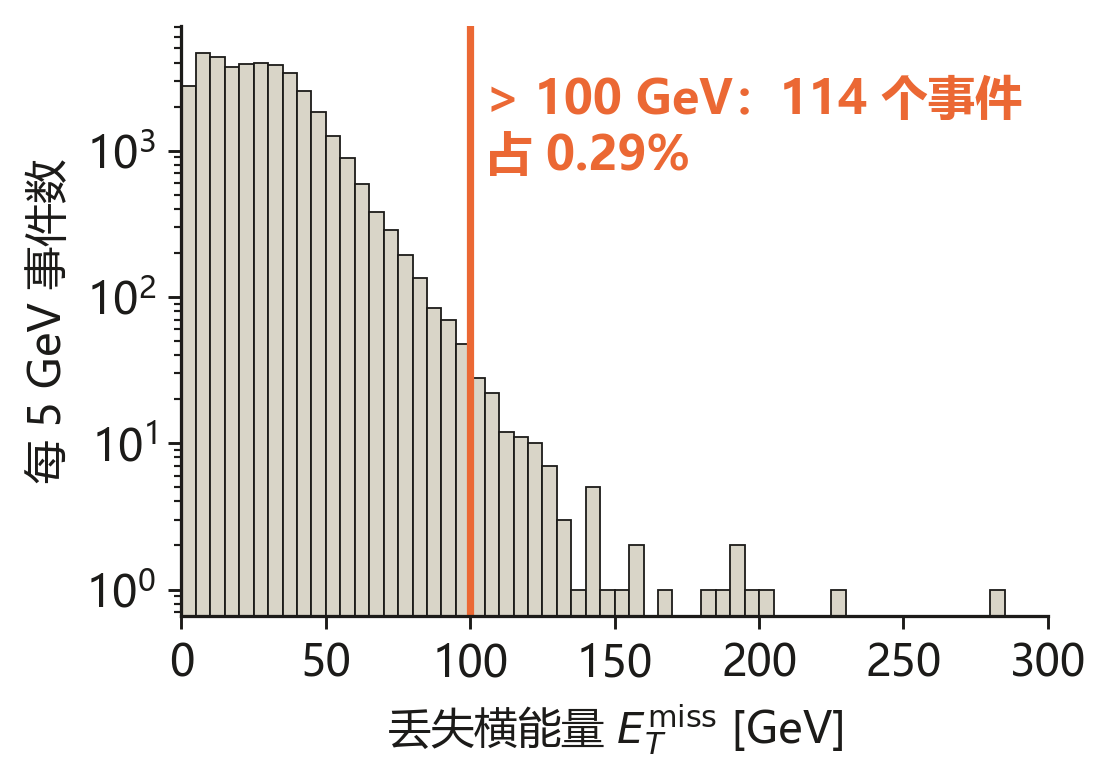
\includegraphics[height=42mm]{met.png}\par
    \end{column}
  \end{columns}
  \vspace{1.5mm}
  {\small\textbf{mono-Z 的思路：}$Z\to\ell\ell$ 再加上大的丢失横能量。重建 Z 是第一步。\\
  \hl{这张图不是搜寻：}没有本底估计，也没校验 $E_{\mathrm{T}}^{\mathrm{miss}}$，不能把尾巴读成信号。\par}
\end{frame}

% 12 --------------------------------------------------------------------
\begin{frame}{留给讨论的三个问题}
  \vspace{7mm}
  \qitem{1}{如果只能选一个 $\pT$ 阈值，你选多少？判断标准是什么？}
  \qitem{2}{没有模拟时，我们能声称“信噪比变好了”吗？}
  \qitem{3}{峰位低了 0.41 GeV。如果只能先查一件事，你查什么？}
\end{frame}

% 备用页 -----------------------------------------------------------------
\begin{frame}{备用：阈值扫描结果}
  \vspace{3mm}
  \centering\small
  \begin{tabular}{rrrrccc}
    \toprule
    $\pT^{\mathrm{cut}}$ [GeV] & 事件数 & 保留比例 & 峰 bin [GeV] & $m_{\mathrm{fit}}$ [GeV] & $\sigma$ [GeV] & $\chi^2/\mathrm{ndf}$\\
    \midrule
    无 & 43493 & 1 & 90.5 & $90.78\pm0.02$ & $1.68\pm0.04$ & 17.1/7\\
    25 & 34023 & 0.782 & 90.5 & $90.83\pm0.03$ & $1.66\pm0.04$ & 13.4/7\\
    30 & 28150 & 0.647 & 90.5 & $90.88\pm0.03$ & $1.66\pm0.04$ & 12.9/7\\
    40 & 11016 & 0.253 & 91.5 & $91.21\pm0.05$ & $1.74\pm0.10$ & 17.8/7\\
    45 & 2385 & 0.055 & 93.5 & $92.66\pm0.22$ & $1.95\pm0.26$ & 2.1/7\\
    \bottomrule
  \end{tabular}\par
  \vspace{5mm}\raggedright
  \smallnote{第一个文件的全部事件，70--109 GeV。拟合 85--97 GeV：Voigt（$\Gamma_Z$ 固定）加指数本底。误差仅含统计部分，各行事件是嵌套子集，并不独立。}
\end{frame}

\begin{frame}{备用：拟合范围的影响}
  \vspace{3mm}
  \centering\small
  \begin{tabular}{lccc}
    \toprule
    拟合范围 [GeV] & $m_{\mathrm{fit}}$ [GeV] & $\sigma$ [GeV] & $\chi^2/\mathrm{ndf}$\\
    \midrule
    87--95 & $90.72\pm0.17$ & $1.80\pm0.32$ & 4.2/3\\
    85--97（主拟合） & $90.78\pm0.02$ & $1.68\pm0.04$ & 17.1/7\\
    80--102 & $90.69\pm0.02$ & $1.84\pm0.02$ & 85.2/17\\
    75--105 & $90.63\pm0.02$ & $1.92\pm0.02$ & 272.4/25\\
    \bottomrule
  \end{tabular}\par
  \vspace{5mm}\raggedright
  \smallnote{峰位随范围变化约 0.15 GeV，大于统计误差。这是粗略的拟合模型差异，不是完整的系统误差。范围越宽，$\chi^2$ 越差，因为模型不含低质量拖尾。}
\end{frame}

\begin{frame}{备用：同号 μ 子不该有 Z 峰}
  \vspace{1mm}
  \centering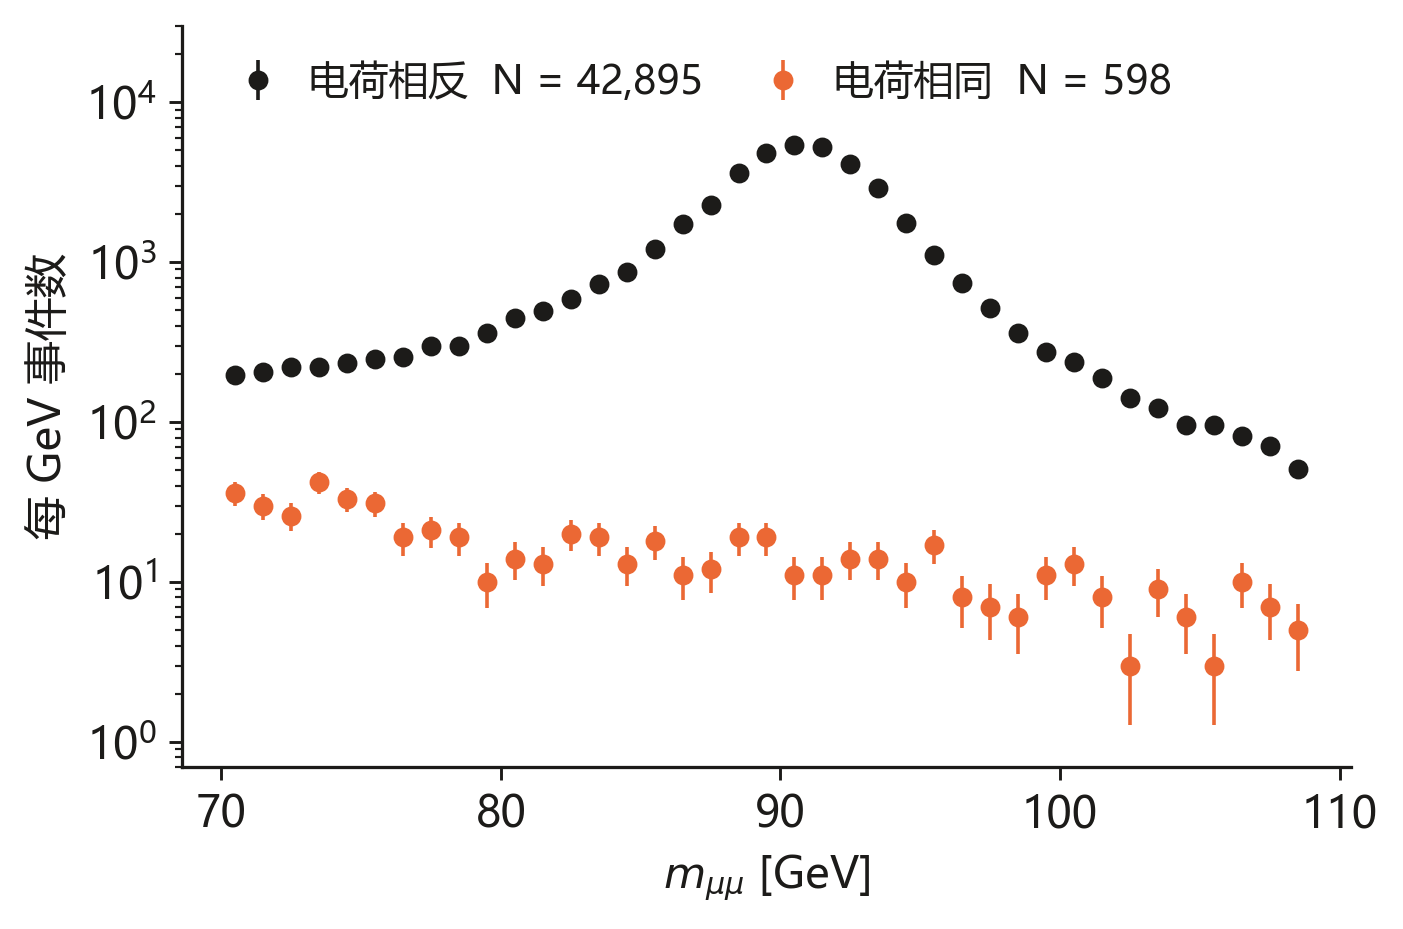
\includegraphics[height=52mm]{charge.png}\par
  \vspace{2mm}\raggedright
  \smallnote{Z 是电中性的，衰变出的两个 μ 子电荷相反。同号事件占窗口内 1.4\%，在 Z 峰位置没有明显的峰。}
\end{frame}

\end{document}
